\section{Investigación}

\subsection{Explique cuál es el entorno y la situación donde se plantea el problema (Motivación)}

MapReduce y su implementación open-source \textit{Hadoop} fueron originalmente optimizadas para grandes lotes de trabajo (batch jobs), como la creación de un índice web. Sin embargo, otro caso de uso surgió recientemente: compartir un cluster MapReduce entre varios usuarios, los cuales ejecutan una mezcla entre grandes lotes de trabajo y pequeñas queries interactivas sobre un conjunto de datos en común. Compartir permite utilizar multiplexación estadística, la cual reduce los costos y, además, conduce a la consolidación de los datos. Esto evita la costosa replicación de los datos a través de clusters privados y permite a una organización ejecutar queries no anticipadas a través de conjuntos de datos disjuntos eficientemente.

La motivación original surge a partir de la carga de trabajo MapReduce en Facebook. Los registros de eventos del sitio web de Facebook son importados a un cluster Hadoop cada hora, donde son utilizados para una variedad de aplicaciones, incluyendo análisis en los patrones de uso para mejorar el diseño del sitio web, detectar spam, data mining, etc.

La central de datos de Facebook corre en 600 máquinas y almacena 500 TB de información comprimida, la cual crece a un promedio de 2 TB por día. Además de los trabajos de \textit{producción} que se deben ejecutar periódicamente, también existen varios trabajos experimentales que van desde cálculos de machine-learning de varias horas hasta queries ad-hoc enviadas cada 1 o 2 minutos a través de una interfaz SQL. Este sistema ejecuta 3200 trabajos MapReduce por día y ha sido utilizado por más de 50 ingenieros de Facebook.


\subsection{Identifique situaciones donde el problema se dispara y la consecuencias que esto genera}

Cuando varios grupos de trabajo comienzan a utilizar Hadoop, el tiempo de respuesta de los trabajos comienzan a sufrir debido al scheduler FIFO que este utiliza. Esto es inaceptable para los trabajos de producción y hace las queries interactivas imposibles, reduciendo altamente la utilidad del sistema. Algunos grupos consideraron construir un cluster privado para su carga de trabajo, pero esto era demasiado caro e injustificado para muchas aplicaciones.

Por otra parte, debido a la interdependencia que existe entra las tareas Map y Reduce, puede suceder que un trabajo que toma mucho tiempo en ejecutarse reserve muchos slots para llevar a cabo su etapa de Reduce, los cuales no liberará hasta haber acabado con su fase Map, produciendo así inanición en otros trabajos y desperdiciando recursos.


\subsection{Identifique del problema}

Los algoritmos tradicionales de scheduling pueden desempeñarse muy pobremente en MapReduce degradando el throughput y el tiempo de respuesta debido a dos aspectos de este: la necesidad de la localidad de los datos (procesar los datos en donde estos se encuentran) y la dependencia entre las tareas Map y Reduce. Estos dos aspectos diferencian el scheduling en clusters MapReduce del scheduling en clusters tradicionales. 


\subsection{Comente el background histórico del problema}

El scheduler integrado de Hadoop ejecuta trabajos en orden FIFO, con cinco niveles de prioridad. La desventaja de un scheduler FIFO es el pobre tiempo de respuesta para trabajos cortos en presencia de trabajos que consumen mucho tiempo. La primer solución para este problema en Hadoop fue Hadoop On Demand (HOD), el cual provee clusters MapReduce privados sobre un gran cluster físico utilizando Torque. HOD permite a los usuarios compartir un sistema de archivos en común (corriendo en todos los nodos) mientras poseen un cluster MapReduce privado en su nodo asignado. Sin embargo, HOD tiene dos problemas:
\begin{itemize}
	\item \textbf{Pobre localidad}: Cada cluster privado corre en un conjunto definido de nodos, pero los archivos HDFS (sistema de archivos que utiliza Hadoop) están distribuidos a través de todos los nodos. Como resultado, algunos Maps deben leer datos a través de la red, degradando el rendimiento y el tiempo de respuesto.
	\item \textbf{Pobre utilización}: Como cada cluster privado tiene un tamaño fijo, algunos nodos en el cluster físico pueden estar inactivos. Esto es subóptimo ya que los trabajos en Hadoop son \textit{elásticos}, en el sentido de que estos pueden cambiar en el tiempo en cuántos nodos se están ejecutando. Los nodos inactivos podrían así incrementar la velocidad a la que se ejecutan los trabajos.
\end{itemize}


\subsection{Explique otros problemas asociados a la búsqueda de una mejor solución}

\begin{center}
	\textbf{Localidad de datos}
\end{center}

El primer aspecto de Map Reduce que plantea retos de scheduling es la necesidad de colocar cálculos cerca de los datos. Esto aumenta el rendimiento porque el ancho de banda de la red de bisección es mucho más pequeño en un clúster grande que el ancho de banda total de los discos del clúster. Ejecutar sobre un nodo que contiene los datos (localidad de nodos) es más eficiente, pero cuando esto no es posible, ejecutar sobre un mismo rack (localidad de racks) provee mejor performance que utilizar un rack no local. Por ejemplo, los nodos de Facebook poseen cuatro discos con un ancho de banda de 50 a 60 MB/s cada uno o 2 GB/s en total, mientras que las conexiones al rack son de 1 GB/s
 
El primer problema de localidad se vio con trabajos pequeños. Es causado por un comportamiento denominado \textit{head-of-line scheduling}. En cualquier momento, hay un único trabajo que debe ser el proximo en ser ejecutado, de acuerdo con \textit{Fair sharing}: el trabajo con el que menos justo se fue. Cualquier esclavo que solicite una tarea se le otorga una a través de ese trabajo. Sin embargo, si el trabajo head-of-line es pequeño, la probabilidad de que los bloques de entrada de un esclavo solicitando una tarea estén disponibles es baja.

Un problema relacionado, \textit{sticky slots} (slots pegajosos), sucede incluso con trabajos largos si se usa ecuanimidad. Por ejemplo si hay 10 trabajos en uno cluster de 100 nodos con un slot por nodo y cada uno corre 10 tareas. Supongamos que el trabajo 1 finaliza una tarea en el nodo X. El Nodo X envía una señal solicitando una nueva tarea. En este punto, el trabajo 1 tiene 9 tareas corriendo mientras todos los otros trabajos tienen 10. Por lo tanto, el trabajo 1 es asignado al nodo X de nuevo. En consecuencia, en estado estable, los jobs nunca dejan sus slots originales. Esto conduce a una mala localidad como en HOD, porque los archivos de entrada son distribuidos a través del cluster. La localidad puede ser  incluso menor con pocos trabajos. Incluso con 5 trabajos, la localidad está por debajo del 50\%.\\

\begin{center}
	\textbf{Interdependencia entre Reduce/Map}
\end{center}
 
En adición a la localidad, otro aspecto de MapReduce que crea retos en el sheduling es la dependencia entre las fases de Map y Reduce. Las fases Map generan resultados intermedios que son almacenados en disco. Cada Reduce copia su porción de resultados de cada Map, y solamente puede aplicar la función de reducción del usuario una vez que se cuenta con los resultados de todos los Maps. Esto puede llevar a un problema de \textit{acaparamiento de los slot} donde los trabajos largos mantienen los slots de Reduce durante mucho tiempo, haciendo que los trabajos pequeños sufran de inanición y se subutilizen recursos.

El primer problema de scheduling de Reduce ocurre en Fair sharing cuando hay trabajos grandes que se ejecutan en el cluster. Hadoop normalmente lanza tareas de Reduce de un trabajo tan pronto como terminan sus primeros Maps, por lo que los Reduce pueden empezar a copiar salidas de Map mientras que los Map restantes se están ejecutando. Sin embargo, en un trabajo grande, de decenas de miles de tareas de Map, la fase de Map puede tardar mucho en completarse. El trabajo retendrá cualquier slot de Reduce que reciba hasta que finalicen todos sus Map. Esto significa que si hay periodos de baja actividad de otros usuarios, el trabajo grande se hará cargo de la mayor parte o de la totalidad de los slots de Reduce en el cluster, y si cualquier trabajo se presenta más tarde, este trabajo sufrirá de inanición hasta que termine el trabajo grande.

Este problema también afecta al rendimiento. En muchos trabajos grandes, las salidas de los Map son pequeñas, debido a que los Map están filtrando un conjunto de datos. Por lo tanto, las tareas Reduce que ocupan slots estarán, mayormente, ociosas a la espera de que terminen los Maps. Sin embargo, un slot Reduce completo es asignado a estas tareas, ya que su fase de computo será costosa una vez que termine su fase de copiado. El trabajo efectivamente \textit{reserva} slots para una futura operación intensiva en el uso del CPU o de la memoria, pero durante el tiempo que los slots están reservados, otros trabajos podrían haber aprovechado el CPU o la memoria para realizar sus propias operaciones.

Puede parecer que estos problemas pueden resolverse comenzando tareas de reduce más tarde o haciéndolas pausables. El problema es que dos operaciones con distintas necesidades de recursos – una copia intensiva en IO y un Reduce intensivo en CPU – se agrupan en una sola tarea. En cualquier momento, un slot de reduce esta o bien utilizando la red para copiar salidas de Map o esta usando el CPU para aplicar la función de Reduce, pero no ambos. Esto puede degradar el rendimiento en un solo trabajo con múltiples oleadas de tareas de Reduce pues hay una tendencia a reducir Reduces a copiar y calcular de forma sincronizada. Cuando los Maps de los trabajos terminan, la primera ola de tareas Reduce comienzan a computar casi simultáneamente, y luego terminan en más o menos el mismo tiempo y la próxima ola empieza a copiar, y así sucesivamente. En cualquier momento, todos los slots están copiando o todas están computando. El trabajo correría mas rápido superponiendo la utilización de IO y CPU (continuar copiando mientras que la primera oleada está computando).


\subsection{Explique las soluciones propuestas}

Para solucionar los problemas se desarrolló el \textbf{scheduler FAIR}. Este scheduler tiene dos metas principales:
\begin{itemize}
	\item \textbf{Aislamiento}: Darle a cada usuario (trabajo) la ilusión de poseer (correr) un cluster privado.
	\item \textbf{Multiplexación estadística}: Redistribuir la capacidad no utilizada por algunos usuarios (trabajos) a otros usuarios (trabajos).
\end{itemize}

FAIR utiliza una jerarquía de dos niveles. En el nivel más alto, FAIR asigna slots de tareas a través de \textit{conjuntos}, y en el segundo nivel, cada conjunto asigna sus slots entre los múltiples trabajos que contiene. Este modelo puede ser fácilmente extendido a más niveles.

FAIR utiliza una versión de max-min fairness con garantías mínimas para asignar slots a través de los conjuntos. A cada conjunto $i$ se le otorga una cuota mínima $m_i$ de slots, la cual puede ser cero. El scheduler se asegura de que cada conjunto reciba su cuota mínima de slots, siempre y cuando tenga suficiente demanda, y la sumatoria sobre todas las cuotas mínimas de slots de cada conjunto no exceda la capacidad del sistema. Cuando un conjunto no utiliza completamente su cuota de slots, otros conjuntos tienen permitido utilizar los que este no utilice.\\

\begin{center}
	\textbf{Delay scheduling}
\end{center}
Para solucionar el problema de la localidad de los datos se utilizó una técnica simple denominada \textit{Delay scheduling}. Cuando un nodo solicita una tarea, si el trabajo no puede lanzar una tarea local, se lo saltea y se pasa a ver los trabajos subsecuentes. Sin embargo, si un trabajo a sido salteado durante un tiempo determinado, se le permite lanzar una tarea no local, evitando así la inanición.\\

\begin{center}
	\textbf{Copy-compute splitting}
\end{center}
Para solucionar los problemas generados por la dependencia entre las fases Map y Reduce, se propuso dividir las tareas Reduce en dos tareas lógicas: tareas de copia y tareas de cómputo, cada cual con una forma diferente de control de admisión, es decir, cada nodo posee slots de copia y slots de cómputo para la fase de Reduce. Las tareas de copia buscan y combinan la salida de las tareas Map, una operación que normalmente está ligada a realizar IO en la red. Las tareas de cómputo aplican la función Reduce del usuario a la salida de las tareas Map.\\


La última complicación generada por la interdependencia entre las fases Map y Reduce es el espacio en disco utilizado por los resultados intermedios (salida de la fase Map). Hadoop ya cuenta con mecanismos de seguridad para asegurarse de que los discos de los nodos no se llenen. Sin embargo, es posible que se produzca un Deadlock si dos trabajos se ejecutan concurrentemente y el disco se llena antes de que alguno de los dos termine. Para evitar este problema, los resultados de uno de los trabajos deben ser eliminados hasta que el otro trabajo termine. Cualquier heurística para elegir que trabajo desalojar sirve siempre y cuando permita a algún trabajo en el cluster avanzar en su progreso. Algunas opciones son:
\begin{itemize}
	\item Desalojar al último trabajo que llegó.
	\item Desalojar al trabajo con el menor porcentaje de progreso.
\end{itemize}

Sin embargo, hay una heurística que no funciona: Desalojar al trabajo que esta utilizando mas espacio del disco. Este método puede llevar a una situación donde los nuevos trabajos que llegan desalojan a los trabajos viejos, y ningún trabajo termina nunca.
    

\subsection{Evalué soluciones propuestas}

Para evaluar la técnicas de scheduling sea realizaron macrobenchmarks y microbenchmarks en tres ambientes diferentes: \textit{Amazon Elastic Compute Cloud} (EC2), que es un entorno virtualizado de hosting comercial, un cluster de 100 nodos (SPC) y un cluster de 450 nodos (LPC).

\begin{figure}[H]
\begin{center}
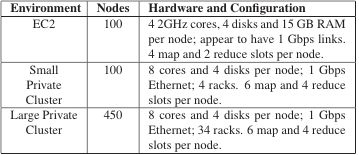
\includegraphics[width=0.6\textwidth]{img/img1.png}
     \caption{Entornos utilizados}
\end{center}
\end{figure}

Para las cargas de trabajo se utilizó \textit{Loadgen}. Loadgen es un trabajo configurable donde las tareas Map devuelven un keepMap\% de los datos datos de entrada, luego las tareas Reduce devuelven un keepReduce\% de los datos intermedios.


\subsubsection{Macrobenchmark}

Se ejecutó un benchmark multiusuario con tamaños de trabajo y tiempos de llegada basados en la carga de trabajo de Facebook. El benchmark utiliza trabajos loadgen con valores al azar para keepMap y keepReduce, y tiempos de uso de CPU al azar (los Maps toman entre 9 y 60 segundos). Este benchmark, referido como BM a partir de ahora, consiste de 50 trabajos de 9 tamaños (números de Maps). La siguiente tabla muestra la distribución de los tamaños en Facebook, la cual fue agrupada en 9 grupos.

\begin{figure}[H]
\begin{center}
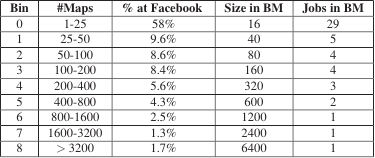
\includegraphics[width=0.6\textwidth]{img/img2.png}
     \caption{Grupos de trabajos}
\end{center}
\end{figure}

Se eligió un tamaño representativo para cada grupo y se envió algún numero de trabajos de dicho tamaño para hacer más fácil el promediar el rendimiento de estos trabajos. Para cada trabajo, se estableció el número de Reduces entre un 5\% y un 25\% del número de Maps. Se envió los trabajos cada 30 segundos aproximadamente, siguiendo un proceso de Poisson, correspondiente al ritmo de envíos en Facebook.

Se generaron tres órdenes de envío de los trabajos de acuerdo a este modelo y se compararon cinco algoritmos de scheduling: FIFO y Fair sharing con y sin copy-compute splitting, así como Fair sharing con ambos copy-compute splitting y delay scheduling.
    
\begin{figure}[H]
\begin{center}
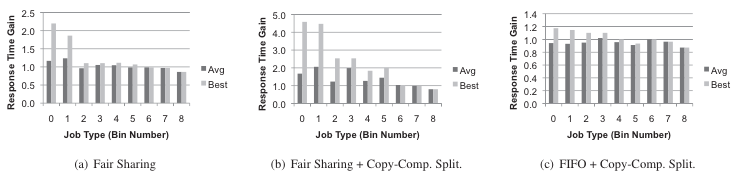
\includegraphics[scale=0.67]{img/img3.png}
     \caption{Ganancia promedio y mejor ganancia en tiempo de respuesta obtenidas por los trabajos de cada grupo en los diferentes algoritmos}
\end{center}
\end{figure}

La figura muestra el tiempo de respuesta promedio ganado por cada tipo (bin) de trabajos por sobre su tiempo de respuesta en FIFO (por ejemplo, un valor 2 indica que el trabajo se ejecutó 2x más rápido que en FIFO), así como la máxima ganancia para cada grupo (la ganancia del trabajo que mejoró más). Se puede ver qué Fair sharing (figura (a)) puede acortar los tiempos de respuesta a la mitad en comparación con FIFO en los trabajos pequeños, a expensa de que los trabajos más largos tomen un poco mas. Sin embargo, algunos trabajos aún son demorados debido al acaparamiento de slots Reduce. Fair sharing con copy-compute splitting (figura (b)) provee ganancias de hasta 4.6x para trabajos pequeños, con el promedio ganado para los trabajos del tipo 0 y 1 siendo de 1.8-2x.
Finalmente, FIFO con copy-compute splitting (figura (c)) produce algunas ganancias pero menos que Fair sharing.

Añadiendo delay scheduling no cambia el tiempo de respuesta de Fair sharing con copy-compute splitting de forma perceptible. Sin embargo, incrementa la localidad de 15-95\% a 99-100\% como se muestra en la siguiente figura (los valores para FIFO, Fair sharing, etc fueron similares, de modo que sólo se muestra un gráfico). Esto incrementa el rendimiento en un entorno con un ancho de banda más limitado que el de EC2 (el cual posee un ancho de banda de 1 GB).

\begin{figure}[H]
\begin{center}
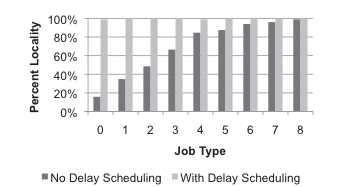
\includegraphics[width=0.6\textwidth]{img/img4.png}
     \caption{Localidad obtenida por cada grupo de trabajos}
\end{center}
\end{figure}

\subsubsection{Microbenchmark}


\begin{center}
	\textbf{Delay scheduling con trabajos pequeños}
\end{center}

Para testear el efecto de delay scheduling sobre la localidad y el rendimiento cuando se utilizan trabajos con poca carga de trabajo, se generó un gran conjunto de datos al azar y se corrió los trabajos sobre el en el entorno SPC. Cada trabajo es solamente un \textit{scan}, es decir, un Map que lee un archivo y retorna un 0.5\% de los datos en el, simulando los comunes trabajos de filtrado cuando se analizan logs. Se ejecutaron trabajos con 3, 10 y 100 tareas Map. El benchmark ejecuta varios números de trabajos basado en el tamaño de los trabajos. Se compararon Fair sharing y FIFO con y sin delay scheduling. FIFO se desempeñó igual que Fair sharing, de modo que solo se mostraran dos barras.

\begin{figure}[H]
\begin{center}
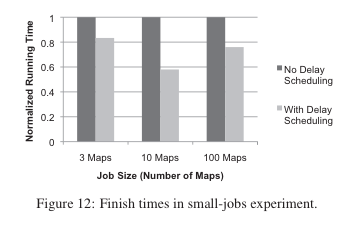
\includegraphics[width=0.6\textwidth]{img/img5.png}
     \caption{Tiempos de ejecución para el experimento con trabajos pequeños}
\end{center}
\end{figure}

\begin{figure}[H]
\begin{center}
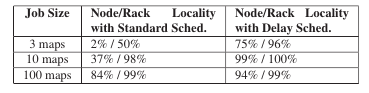
\includegraphics[width=0.6\textwidth]{img/img6.png}
     \caption{Localidad conseguida en el experimento con trabajos pequeños}
\end{center}
\end{figure}

Los gráficos muestran los tiempos de ejecución normalizados de los trabajos, mientras que la tabla 3 la localidad conseguida por cada scheduler. Delay scheduling incrementó el rendimiento \textbf{1.2x} en trabajos con 3 Maps, \textbf{1.7x} en trabajos con 10 Maps y \textbf{1.3x} en trabajos con 100 Maps, e incrementó la localidad de los datos al menos a un \textbf{75\%} y la localidad en los rack a al menos un \textbf{94\%}. El rendimiento ganado es mayor para los trabajos con 10 Maps que para los trabajos con 100 Maps debido a que la localidad en los trabajos con 100 Maps es bastante buena, incluso sin delay scheduling. Sin embargo, la ganancia para los trabajos más pequeños (3 Maps) es menor que para los trabajos con 10 Maps, debido a que los trabajos de pequeño tamaño al inicializarse producen un cuello de botella en Hadoop.\\


\begin{center}
	\textbf{Delay scheduling con sticky slots}
\end{center}

Sticky slots no ocurre en Hadoop debido a un bug en este, de modo que se arregló este bug para poder medir los efectos de sticky slots.

Este test se corrió en el entorno EC2. Se generó un gran conjunto de datos de 180 GB (2 GB por nodo), se envío entre 5 y 50 trabajos \textit{scan} concurrentes y se midió el tiempo que tardaron en terminar todos los trabajos y la localidad conseguida. Los siguientes gráficos muestran los resultados obtenidos con y sin delay scheduling. 

\begin{figure}[H]
\begin{center}
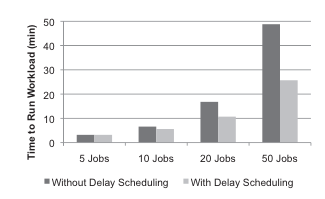
\includegraphics[width=0.6\textwidth]{img/img7.png}
     \caption{Tiempos de ejecución en el experimento de sticky slots}
\end{center}
\end{figure}

\begin{figure}[H]
\begin{center}
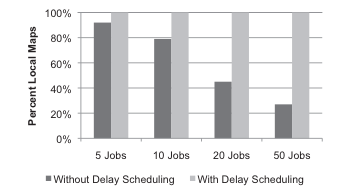
\includegraphics[width=0.6\textwidth]{img/img8.png}
     \caption{Localidad de nodos conseguida en el experimento de sticky slots}
\end{center}
\end{figure}

Delay scheduling incrementó el rendimiento en \textbf{1.1x} para 10 trabajos concurrentes, \textbf{1.6x} para 20 trabajos concurrentes y \textbf{2x} para 50 trabajos concurrentes. También incrementó la localidad de \textbf{27-90\%} hasta \textbf{99-100\%}.\\


\begin{center}
	\textbf{Impacto de delay scheduling en el tiempo de respuesta}
\end{center}

Se midió el tiempo de respuesta de un pequeño trabajo con 16 Maps y 1 Reduce (escaneando 2 GB y enviando \textbf{0.1\%} de los datos al Reduce) con y sin delay scheduling en el entorno EC2 para cuantificar el impacto en el tiempo de respuesta. Se ejecutó al trabajo ocho veces sobre cada condición. Ejecutándose sólo, el trabajo tomo 32 a 37 segundos, con una media de 35.4 segundos. Con delay scheduling, el trabajo tomo 32 a 38 segundos, con una media de 35.a segundos. La diferencia en los tiempos de respuesta no fue estadísticamente significativa, pero la localidad mejoró de un \textbf{25\%} a un \textbf{100\%}.\\


\begin{center}
	\textbf{Copy-compute splitting con un solo trabajo}
\end{center}

Desafortunadamente, las tareas de copia en Hadoop son bastante intensivas en el uso del CPU ya que estas realizan grandes cantidades de copias en memoria cuando combinan las salidas de los Maps, así que hay poca ganancia por parte de copy-compute splitting a menos que el ancho de banda de la red sea muy limitado (las tareas de copia compiten con las tareas de cómputo por el CPU). En el entorno LPC se ejecutó un trabajo con una función identidad en Map y una función Reduce intensiva en CPU. El trabajo tomo 1.8 TB de datos de entrada. 14624 tareas Map y 5000 tareas Reduce. Los Reduce corrieron en tres oleadas, ya que el cluster está configurado con 1800 slots de Reduce (cuatro por nodo). El trabajo tomó, en promedio, 12.9 minutos con el scheduler de Reduce estándar y 11.8 minutos con copy-compute splitting, una ganancia del 9\%. Se espera que la ganancia sea mayor en clusters más grandes o con una implementación más eficiente de las tareas de copia.\\


\begin{center}
	\textbf{Tiempo de respuesta Batch con Fair sharing vs FIFO}
\end{center}

Se ejecutaron cinco trabajos en el entorno EC2. Cada trabajo lee 100 GB de datos. Los Maps del trabajo producen 200 GB de salida, en total. Estos datos son pasados a 190 tareas Reduce. Las tareas Reduce devuelven solo un pequeño conjunto pero realizan intensivos cálculos matemáticos por cada documento. Se repitió el experimento tres veces. Fair sharing tomo 25.9 a 26.5 minutos en completar el trabajo, mientras que FIFO tomo 21.9 a 22.3 minutos. Esto corresponde a un rendimiento \textbf{19\%} mayor con FIFO.


\subsection{Discusión}

Se identificaron dos aspectos que plantean problemas de los cluster que llevan a cabo cómputo intensivo en datos: la localidad de los datos y la interdependencia de las tareas. Cualquier sistema que coloque las tareas en los nodos que contienen los datos necesarios corre el riesgo de sufrir los problemas descritos: \textit{head-of-line scheduling} y \textit{sticky slots}. Similarmente, son comunes las tareas que deben recolectar datos de múltiples otras tareas antes de poder realizar su cómputo. Las técnicas de \textit{delay scheduling} y \textit{copy-compute splitting} pueden mejorar el rendimiento y el tiempo de respuesta en cualquier sistema basado en flujo de datos.\\

\begin{center}
	\textbf{Lecciones para scheduling en clusters multiusuario}
\end{center}

Siempre que los trabajos estén compuestos de pequeñas tareas independientes, es posible aislar a los usuarios mientras que se utiliza el cluster eficientemente. Se identificaron cuatro principios que ayudan a alcanzar esta meta:
\begin{itemize}
	\item Hacer las tareas pequeñas en duración y en consumo de recursos. Tener tareas cortas permite a los nuevos trabajos comenzar más rápido. Limitar los recursos de cada tarea (por ejemplo, haciendo que las tareas utilicen un único thread y teniendo múltiples slots por nodo) incrementa las oportunidades de scheduling.
	\item Dividir las tareas en partes con requerimientos ortogonales de recursos para tener diferentes controles de admisión para cada tarea.
	\item Cuando las tareas deben ser largas, también deben ser desalojables.
	\item Estar preparado para sacrificar algo de aislamiento a cambio de rendimiento, como lo ilustra delay scheduling.
\end{itemize}


\begin{center}
	\textbf{Schedulers para MapReduce:}
\end{center}

Si comparamos los schedulers: FIFO, Fair sharing, SJF y colas multi-nivel (colas separadas para trabajos largos y cortos, con Fair sharing ponderado entre las colas); y utilizamos las métricas: tiempo de respuesta promedio, tiempo de respuesta batch (tiempo de respuesta para un grupo de trabajos que llegan a la vez), espacio intermedio y aislamiento de usuarios (definido como la habilidad de proveer al usuario un rendimiento similar al de un pequeño cluster privado en el peor caso, sin importar su carga de trabajo); se obtienen tres resultados interesantes:
\begin{itemize}
	\item El tiempo de respuesta Batch sufre en todos los schedulers menos en FIFO, ya que los Maps pueden terminar más tarde y, por lo tanto, el pipelining entre las tareas Map y Reduce sufre.
	\item FIFO utiliza el menor espacio intermedio (no más que el necesario por el trabajo más grande), mientras que los que permiten a varios trabajos coexistir necesitan más espacio. Con SJF la cantidad de espacio utilizado puede ser arbitrariamente grande ya que muchos trabajos pueden estar en el sistema por un periodo arbitrariamente largo.
	\item Sólo Fair sharing provee aislamiento de usuarios (incluso en colas multi-nivel, el trabajo de un usuario puede ser retrasado por otros usuarios)
\end{itemize}

Aunque Fair sharing es subóptimo en tiempo de respuesta y utilización de espacio, hemos encontrado que el aislamiento de usuarios supera a estas preocupaciones mediante la creación de un ambiente donde los usuarios pueden iniciar trabajos en cualquier momento sin temor a interferencias. Un beneficio de que los usuarios puedan lanzar trabajos inmediatamente es que permite que la detección de bugs sea mas rápida: sin Fair sharing, un usuario que envía un trabajo con un Map o Reduce buggeados no lo detectara hasta que este alcance la primer posición de la cola y sea lanzado.

\begin{center}
	\textbf{Otros problemas de scheduling}
\end{center}

\begin{itemize}
	\item \textbf{Localidad de código}: Ejecutar múltiples tareas de un trabajo en un nodo es beneficioso ya que amortiza el costo de tener copiar el código del trabajo. El problema de maximizar la localidad de código es similar a scheduling por afinidad en los sistemas operativos multiprocesador, donde se intenta que un thread se ejecute en un mismo procesador por todo el tiempo posible.
	\item \textbf{Gestión de la carga de los esclavos}: Cuando trabajos con diferentes requisitos de recursos (especialmente de memoria) coexisten, podría ser beneficioso utilizar un mecanismo más elaborado que slots de tareas para manejar la carga en los nodos esclavos. Sin embargo, otro problema que puede darse es inanición para los procesos intensivos en el uso de la memoria si trabajos con menores requisitos de memoria ocupan los slots.
\end{itemize}

\subsection{Conclusiones}

Mientras que MapReduce ha probado ser un modelo popular para ejecutar grandes lotes de trabajos, recientemente, muchas organizaciones han comenzado a compartir su cluster MapReduce (Hadoop) entre múltiples usuarios, los cuales ejecutan una mezcla de lotes de trabajos y pequeños trabajos interactivos. Para habilitar este modelo, se ha propuesta a FAIR, un scheduler que provee aislamiento, garantiza una cuota mínima para cada usuario (trabajo) y logra multiplexación estadística. En una primera instancia, se han identificado dos aspectos de MapReduce (localidad de los datos e interdependencia entre tareas Map y Reduce) que afectaban considerablemente el rendimiento de FAIR. Para solucionar este problema se desarrollaron dos simples y, a su vez, robustas soluciones: delay scheduling y copy-compute splitting. Utilizando un amplio conjunto de experimentos se demostró que FAIR consigue aislamiento, bajo tiempo de respuesta y alto rendimiento.
